\documentclass[tikz,border=8pt]{standalone}
% Shared look for every TikZ diagram. Load with \input{../../tools/tikz-style.tex}
\usepackage[T1]{fontenc}
\usepackage{lmodern}
\renewcommand{\sfdefault}{lmr}  % diagrams use the same serif as the text
\usetikzlibrary{arrows.meta, positioning, shapes.geometric, calc, fit, backgrounds}
\definecolor{cblue}{HTML}{4C78A8}
\definecolor{corange}{HTML}{F58518}
\definecolor{cgreen}{HTML}{54A24B}
\definecolor{cred}{HTML}{E45756}
\definecolor{cpurple}{HTML}{B279A2}
\definecolor{cgrey}{HTML}{6B6B6B}
\tikzset{
  every picture/.style={font=\sffamily, line width=1.2pt},
  box/.style={draw=#1, fill=#1!12, rounded corners=4pt, align=center, inner sep=7pt, minimum height=1.1cm},
  box/.default=cgrey,
  arrow/.style={-{Stealth[length=3mm]}, draw=cgrey, line width=1.4pt},
  title/.style={font=\sffamily\bfseries\Large},
  note/.style={font=\sffamily\small, text=cgrey, align=center},
}
\AtBeginDocument{\hyphenpenalty=10000 \exhyphenpenalty=10000}

\begin{document}
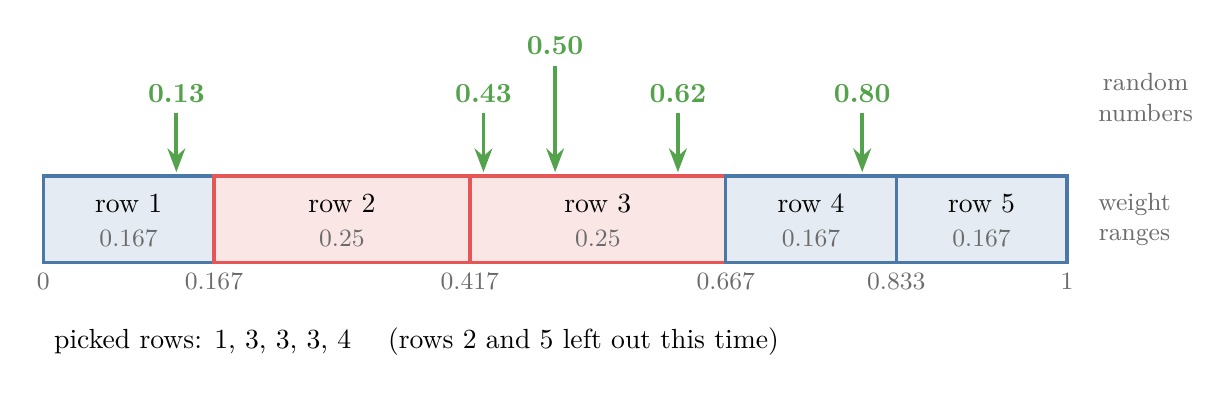
\begin{tikzpicture}[x=13cm]
  \foreach \a/\b/\r/\w/\c in {0/0.1667/1/0.167/cblue, 0.1667/0.4167/2/0.25/cred, 0.4167/0.6667/3/0.25/cred,
                              0.6667/0.8333/4/0.167/cblue, 0.8333/1/5/0.167/cblue} {
    \filldraw[draw=\c, fill=\c!15, line width=1.2pt] (\a,0) rectangle (\b,1.1);
    \node at ({(\a+\b)/2},0.75) {row \r};
    \node[note] at ({(\a+\b)/2},0.3) {\w};
  }
  \foreach \t in {0, 0.1667, 0.4167, 0.6667, 0.8333, 1} \node[note, below] at (\t,0) {\pgfmathprintnumber[fixed, precision=3]{\t}};
  \foreach \u/\h in {0.13/1.9, 0.43/1.9, 0.50/2.5, 0.62/1.9, 0.80/1.9} {
    \draw[arrow, draw=cgreen] (\u,\h) -- (\u,1.15);
    \node[above, text=cgreen, font=\sffamily\bfseries] at (\u,\h) {\u};
  }
  \node[note, anchor=west] at (1.02,2.1) {random\\numbers};
  \node[note, anchor=west] at (1.02,0.55) {weight\\ranges};
  \node[anchor=west] at (0,-1.0) {picked rows: 1, 3, 3, 3, 4 \quad (rows 2 and 5 left out this time)};
\end{tikzpicture}
\end{document}
